\documentclass[a4paper,oneside,12pt]{article}  
\usepackage[utf8]{inputenc}
\usepackage[slovak]{babel}
\usepackage[T1]{fontenc}
\usepackage[pdftex]{graphicx}
\usepackage{mathtools}
\usepackage[european]{circuitikz}
\usepackage{amssymb}
\usepackage{makecell}

\author{Matej Otcenas (xotcen01)}
\date{\today}
\title{Projekt IEL}

\begin{titlepage}
\end{titlepage}

\begin{document}


	\maketitle
	\newpage

\begin{figure}[h]
	\begin{center}
		
\includegraphics[height = 96pt]{fit_pic.png}
	\end{center}
\end{figure}
	
	\tableofcontents
	\newpage
 	\begin{center}

	{\textbf{\LARGE Riešené príklady 2018/19}}
	
	\end{center}
	\maketitle
	\section{Príklad č.1}
	
	\maketitle
	\subsection{Zadanie}
	
	Vypočítaj napätie $U_3$ a prúd $I_3$. Použi metódu postupného zjednodušovania.
	
	
	\begin{table}[h]
		\begin{center}		
			\begin{tabular}{|c|c|c|c|c|c|c|c|c|c|c|}
					\hline
					sk. & $U_{1}$ [$V$] & $U_{2}$ [$V$] & $R_{1}$ [$\Omega$] &  $R_{2}$ [$\Omega$] & $R_{3}$ [$\Omega$] & $R_{4}$ [$\Omega$] & $R_{5}$ [$\Omega$] & $R_{6}$ [$\Omega$] & $R_{7}$ [$\Omega$] & $R_{8}$ [$\Omega$] \\
					\hline
					D & 105 & 85 & 420 & 980 & 330 & 280 & 310 & 710 & 240 & 200 \\
					\hline
			\end{tabular}
		\end{center}
	\end{table}
	
\begin{figure}[h]
		\begin{center}
			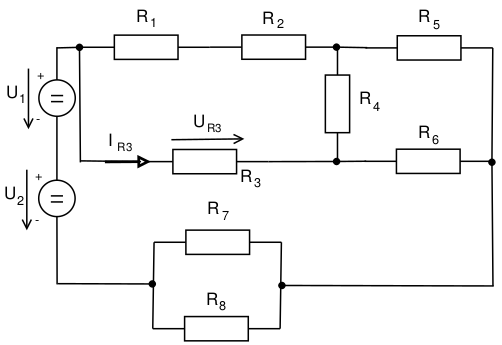
\includegraphics[width=10cm]{circuit_1.png}
		\end{center}
\end{figure}

\maketitle
\subsection{Postup}

1.Obvod postupne zjednodušíme : 
\begin{eqnarray*}
	U &= & U_{1} + U_{2} = 105 + 85 = 190V \\
	R_{12} &= & R_{1} + R_{2} = 980 + 420 = 1400 \Omega\\
	R_{78} &= & R_{7} || R_{8} = \frac{R_{7} * R_{8}}{R_{7} + R_{8}} = \frac{240 * 200}{240 + 200} = 109.0909 \Omega\\ 
\end{eqnarray*}


\begin{center}
	\begin{circuitikz}
		\draw
		
		(0,0) to[R,l=$R_{78}$] (2,0)
		(0,3) to[V,v=$U_{12}$](0,0) 
		(0,3) to[short,-*] (3,3) to[short] (3,1) to [short] (3.5,1) to[R,l=$R_{3}$] (5.5,1) to [short,-*] (6,1) to [short] (6,1.5)
		(3,3) to[short] (3.5,3) to[R,l=$R_{12}$] (5.5,3) to [short, -*] (6,3) to[short] (6,2.5) to[R,l=$R_{4}$] (6,1.5)
		(6,3) to[short] (7,3) to[R,l=$R_{5}$] (9,3) to [short, -*] (9,1)
		(6,1) to[short] (7,1) to[R,l=$R_{6}$] (9,1) to [short] (9,0) to [short] (2,0)
		
		
		;
	\end{circuitikz}
\end{center}


2.Následne prevedieme transfiguráciu $R_{12}$, $R_{3}$, $R_{4}$ z trojuholníka na 

hviezdu a vzniknú nám rezistory $R_{A}$, $R_{B}$, $R_{C}$.
\begin{eqnarray*}
	R_{A} &= & \frac{R_{12} * R_{3}}{R_{12} + R_{3} + R_{4}} = \frac{1400 * 330}{1400 + 330 + 280} = 229.8507 \Omega\\
	R_{B} &= & \frac{R_{12} * R_{4}}{R_{12} + R_{3} + R_{4}} = \frac{1400 * 280}{1400 + 330 + 280} = 195.0249 \Omega\\
	R_{C} &= & \frac{R_{3} * R_{4}}{R_{12} + R_{3} + R_{4}} = \frac{330 * 280}{1400 + 330 + 280} = 45.9701 \Omega\\
\end{eqnarray*}

\begin{center}
	\begin{circuitikz}
		\draw
		(0,0) to[R,l=$R_{78}$] (2,0)
		(0,3) to[V,v=$U_{12}$](0,0) 
		(0,3) to[short] (2,3) to[R,l=$R_{A}$] (4,3) to[short] (5,4) to[R,l=$R_{B}$] (6,4)to[R,l=$R_{5}$] (8,4) to [short,-*] (8,2) 
		(4,3) to[short] (5,2) to[R,l=$R_{C}$] (6,2) to[R,l=$R_{6}$] (8,2) to[short] (8,0) to[short] (2,0) 
		;
	\end{circuitikz}
\end{center}


3.Využijeme sériového zapojenia rezistorov $R_{B}$ + $R_{5}$ a $R_{C}$ + $R_{6}$.
\begin{eqnarray*}
	R_{B5} &= & R_{B} + R_{5} = 195.0249 + 310 = 505.0249 \Omega\\
	R_{C6} &= & R_{C} + R_{6} = 45.9701 + 710 = 755.9701 \Omega\\
\end{eqnarray*}    

\begin{center}
	\begin{circuitikz}
		\draw
		(0,0) to[R,l=$R_{78}$] (2,0)
		(0,3) to[V,v=$U_{12}$](0,0) 
		(0,3) to[short] (2,3) to[R,l=$R_{A}$] (4,3) to[short] (5,4) to[R,l=$R_{B5}$] (6,4) to[short] (7,4) to [short,-*] (7,2) 
		(4,3) to[short] (5,2) to[R,l=$R_{C6}$] (6,2) to[short] (7,2) to[short] (7,0) to[short] (2,0) 
		;
	\end{circuitikz}
\end{center}

4.Tentokrát nám vzniknú dva paralelne zapojené rezistory $R_{B5}$ a $R_{C6}$
\begin{eqnarray*}
	R_{B5C6} &= & R_{B5} || R_{C6} = \frac{R_{B5} * R_{C6}}{R_{B5} + R_{C6}} = \frac{505.0249 * 755.9701}{505.0249 + 755.9701} = 302.7639 \Omega\\
\end{eqnarray*}

\begin{center}
	\begin{circuitikz}
		\draw
		(0,0) to[R,l=$R_{78}$] (2,0)
		(0,3) to[V,v=$U_{12}$](0,0) 
		(0,3) to[short] (2,3) to[R,l=$R_{A}$] (4,3) to[short] (5,3) to[R,l=$R_{B5C6}$] (6,3) to[short] (7,3) to [short] (7,0) to[short] (2,0) 
		
		;
	\end{circuitikz}
\end{center}

5.Znovu zjednodušíme sériovo zapojené rezistory $R_{B5C6}$ a $R_{A}$.
\begin{eqnarray*}
	R_{AB5C6} &= & R_{B5C6} + R_{A} = 302.7639 + 229.8507 = 532.6146 \Omega\\ 
\end{eqnarray*}

\begin{center}
	\begin{circuitikz}
		\draw
		(0,0) to[R,l=$R_{78}$] (2,0)
		(0,3) to[V,v=$U_{12}$](0,0) 
		(0,3) to[short] (2,3) to[R,l=$R_{AB5C6}$] (4,3) to[short] (5,3) to[short] (5,0) to[short] (2,0)
		
		;
	\end{circuitikz}
\end{center}

6.Nakoniec vypočítame $R_{EKV}$ pomocou sériovo zapojených rezistorov 

$R_{AB5C6}$ a $R_{78}$.
\begin{eqnarray*}
	R_{EKV} &= & R_{AB5C6} + R_{EKV} = 532.6146 + 109.0909 = 641.7055 \Omega\\
\end{eqnarray*}

\begin{center}
	\begin{circuitikz}
		\draw
		(0,3) to[V,v=$U_{12}$](0,0) 
		(0,3) to[short] (2,3) to[R,l=$R_{EKV}$] (4,3) to[short] (5,3) to[short] (5,0) to[short] (0,0)
		
		;
	\end{circuitikz}
\end{center}

7.Zistíme celkový prúd $I = \frac{U_{12}}{R_{EKV}}$
\begin{eqnarray*}
	I &= & \frac{190}{641.7055} = 0.2961 \ A \\
\end{eqnarray*}


8.Analogicky sa musím vrátiť naspäť aby som zistil napätie $U_{3}$ a prúd $I_{3}$.

Potrebujem zostaviť rovnicu $U_{R_{3}}$ = $U_{12}$ - $U_{R_{6}}$ - $U_{R_{78}}$
\begin{eqnarray*}
	U_{R_{B5C6}} &= & U_{R_{C6}} = I * R_{B5C6} = 0.2961 * 302.7639 = 89.6484 V \\
	U_{R_{78}} &= & I * R_{78} = 0.2961 * 109.0909 = 32.3018 V \\
\end{eqnarray*}


9.Vypočítam prúd $I_{R_{C6}}$ = $I_{R_{6}}$ aby som mohol vypočítať napätie $U_{R_{6}}$.
\begin{eqnarray*}
	I_{R_{C6}} &= &\frac{U_{R_{C6}}}{R_{C6}} = \frac{89.6484}{755.9701} = 0.1186 A \\
	U_{R_{6}} &= & I_{R_{6}} * R_{6} = 0.1186 * 710 = 84.2060 \Omega\\
\end{eqnarray*}


10.Môžem zostaviť rovnicu z bodu č.8
\begin{eqnarray*}
	U_{R_{3}} &= & U_{12} - U_{R_{6}} - U_{R_{78}} = 190 - 84.2060 - 32.3018 = 73.5019 V \\
	I_{R_{3}} &= & \frac{U_{R_{3}}}{R_{3}} = \frac{73.5019}{330} = 0.2227 A \\ 
\end{eqnarray*}

\maketitle
\subsection{Výsledok}

\begin{eqnarray*}
	U_{R_{3}} &= & 73.5019 V \\
	I_{R_{3}} &= & 0.2227 A \\ 
\end{eqnarray*}

\newpage

\maketitle
\section{Príklad č.2}

\maketitle
\subsection{Zadanie}
Stanovte napätie $U_{R_{1}}$ a prúd $I_{R_{1}}$. Použite metódu Théveninovej vety.

\begin{table}[h]
		\begin{center}		
			\begin{tabular}{|c|c|c|c|c|c|c|}
					\hline
					sk. & $U$ [$V$] & $R_{1}$ [$\Omega$] &  $R_{2}$ [$\Omega$] & $R_{3}$ [$\Omega$] & $R_{4}$ [$\Omega$] & $R_{5}$ [$\Omega$] \\
					\hline
					B & 100 & 50 & 310 & 610 & 220 & 570 \\
					\hline
			\end{tabular}
		\end{center}
	\end{table}
	
\begin{figure}[h]
		\begin{center}
			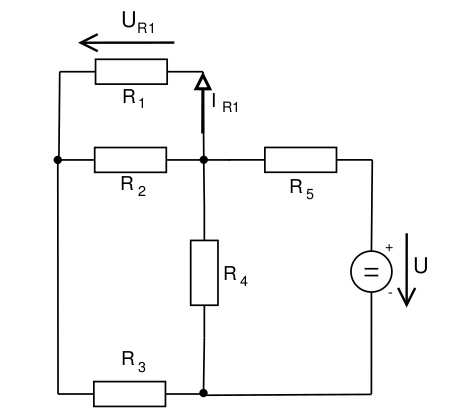
\includegraphics[width=10cm]{circuit_2.png}
		\end{center}
\end{figure}

\maketitle
\subsection{Postup}

1.Odpojíme rezistor $R_{1}$, zdroj $U$ a spočítame vnútorný odpor $R_{i}$ 
\begin{eqnarray*}
	R_{45} &= & R_{4}||R_{5} = \frac{R_{4} * R_{5}}{R_{4} + R_{5}} = \frac{220 * 570}{220 + 570} = 158.7342 \Omega\\
	R_{345} &= & R_{45} + R_{3} = 158.7342 + 610 = 768.7342 \Omega\\
	R_{i} &= & \frac{R_{345} * R_{2}}{R_{345} + R_{2}} = \frac{768.7342 * 310}{768.7342 + 310} = 220.9141 \Omega\\   
\end{eqnarray*}

\begin{center}
	\begin{circuitikz}
		\draw
		(0,0) to[R,l=$R_{3}$] (2,0) to[short,-*] (4,0) to [short] (6,0) to[short] (6,5) to [R,l=$R_{5}$] (4,5) to[short, o-] (3,5) to[short] (2.5,5) to[R,l=$R_{2}$] (1.5,5) to [short, -o] (0,5) to [short] (0,0) 
		(4,0) to[short] (4,2) to[R,l=$R_{4}$] (4,3) to [short] (4,5)		
		;
	\end{circuitikz}
\end{center}

2.Vypočítame prúd $I$ v obvode pomocou celkového odporu $R_{CELK}$
\begin{eqnarray*}
	R_{23} &= & R_{2} + R_{3} = 310 + 610 = 920 \Omega\\
	R_{234} &= & R_{23}||R_{4} = \frac{R_{23} * R_{4}}{R_{23} + R_{4}} = \frac{920 * 220}{920 + 220} = 177.5439 \Omega\\
	R_{CELK} &= & R_{234} + R_{5} = 177.5439 + 570 = 747.5439 \Omega\\
	\\
	I &= & \frac{U}{R_{CELK}} = \frac{100}{747.5439} = 0.1338 A \\
\end{eqnarray*}

3.Vypočítam napätie $U_{THEV} = U_{R_{2}}$, ktoré je na odpore $R_{2}$. Musíme vypočítať $I_{R_{2}}$.
\begin{eqnarray*}
	I_{R_{234}} &= &I \\
	U_{R_{23}} &= &U_{R_{234}} \\
	U_{R_{234}} &= &I * R_{234} = 0.1338 * 177.5439 = 23.7554 V \\
	I_{R_{2}} &= &I_{R_{23}} \\
	I_{R_{2}} &= &\frac{U_{R_{23}}}{R_{23}} = 0.0258 A \\
	U_{THEV} &= & I_{R_{2}} *  R_{2} = 7.998 V\\
\end{eqnarray*}

\begin{center}
	\begin{circuitikz}
		\draw
		(0,0) to[R,l=$R_{3}$] (2,0) to[short,-*] (4,0) to [short] (6,0) to[short] (6,2)
		 (6,3) to[short](6,5)to[R,l=$R_{5}$] (4,5) to[short, o-] (3,5) to[short] (2.5,5) to[R,l=$R_{2}$] (1.5,5) to [short, -o] (0,5) to [short] (0,0) 
		(4,0) to[short] (4,2) to[R,l=$R_{4}$] (4,3) to [short] (4,5)	
		(6,3) to[V,v=$U$] (6,2)	
		(4,5) to[short] (4,6.5) to [open,v=$U_{THEV}$] (0,6.5)
		(0,5) to[short] (0,6.5)
		;
	\end{circuitikz}
\end{center}

4.Pomocou $U_{THEV}$, vnútorného odporu $R_{i}$ a odporu $R_{1}$ je možné stanoviť 

hľadaný prúd $I_{R_{1}}$ a napätie $U_{R_{1}}$
\begin{eqnarray*}
	I_{R_{1}} &= & \frac{U_{THEV}}{R{i} + R_{1}} = \frac{7.998 V}{220.9141 + 50} = 0.0295 A \\
	\\
	U_{R_{1}} &= & R_{1} * I_{R_{1}} = 50 * 0.0295 = 1.475 V \\
\end{eqnarray*}

\begin{center}
	\begin{circuitikz}
		\draw
		(0,3) to[V,v=$U_{THEV}$] (0,1) to [short] (0,0)
		(0,3) to[short] (0,4) to[short](1,4) to[R,l=$R_{i}$] (3,4) to[short] (4,4) to[short] (4,3) to[R,i=$I_{R_{1}}$, l=$R_{1}$] (4,1) to[short] (4,0) to[short] (0,0)
		;
	\end{circuitikz}
\end{center}

\maketitle
\subsection{Výsledok}

\begin{eqnarray*}
	U_{R_{1}} &= & 1.8350 V \\
	I_{R_{1}} &= & 0.0367 A \\ 
\end{eqnarray*}

\newpage

\maketitle
\section{Príklad č.3}

\maketitle
\subsection{Zadanie}
Stanovte napätie $U_{R_{3}}$ a prúd $I_{R_{3}}$. Použite metódu uzlových napätí ($U_{A}$, $U_{B}$, $U_{C}$).


\begin{table}[h]
		\begin{center}		
			\begin{tabular}{|c|c|c|c|c|c|c|c|c|}
					\hline
					sk. & $U$ [$V$] & $I_{1}$ [$A$] & $I_{2}$ [$A$] & $R_{1}$ [$\Omega$] &  $R_{2}$ [$\Omega$] & $R_{3}$ [$\Omega$] & $R_{4}$ [$\Omega$] & $R_{5}$ [$\Omega$] \\
					\hline
					G & 160 & 0.65 & 0.45 & 46 & 41 & 53 & 33 & 29  \\
					\hline
			\end{tabular}
		\end{center}
	\end{table}

\begin{figure}[h]
		\begin{center}
			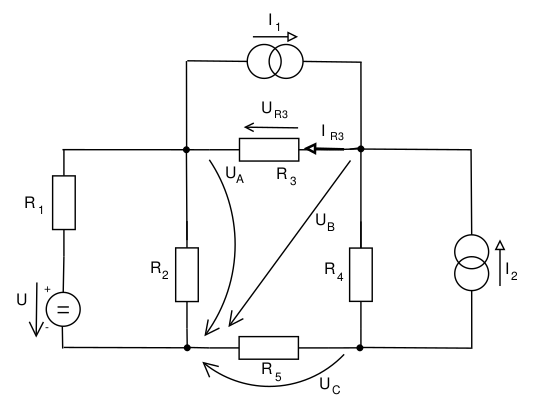
\includegraphics[width=10cm]{circuit_3.png}
		\end{center}
\end{figure}

\maketitle
\subsection{Postup}

1.Zostavíme rovnice pre 3 uzly $A, B, C$ podľa $I.K.Z$
\begin{eqnarray*}
	&A: & I_{R_{1}} - I_{R_{2}} + I_{R{3}} - I_{1} = 0 \\
	&B: & I_{R_{2}} - I_{R_{4}} - I_{R{3}} + I_{1} = 0 \\
	&C: & I_{R_{4}} - I_{R_{5}} - I_{2} = 0 \\
\end{eqnarray*}

2.Jednotlivé odpory vyjadrím cez vodivosť
\begin{eqnarray*}
	G_{1} = \frac{1}{R_{1}} = 0.0217 \Omega\\
	G_{2} = \frac{1}{R_{2}} = 0.0244 \Omega\\
	G_{3} = \frac{1}{R_{3}} = 0.0189 \Omega\\
	G_{4} = \frac{1}{R_{4}} = 0.0303 \Omega\\
	G_{5} = \frac{1}{R_{5}} = 0.0345 \Omega\\
\end{eqnarray*}

3.Rozpíšem rovnice podľa $II.K.Z$ a využijem vodivosť pre zjednodušenie výpočtu
\begin{eqnarray*}
	&A: & G_{1} * (U - U_{A}) + G_{3} * (U_{B} - U_{A}) - G_{2} * U_{A} = I_{1}\\
	&B: & -G_{4} * (U_{B} - U_{C}) - G_{3} * (U_{B} - U_{A}) = -I_{1} - I_{2}\\
	&C: & G_{4} * (U_{B} - U_{C}) - G_{5} * U_{C} = I_{2}\\
\end{eqnarray*}

4.Tieto rovnice môžme upraviť tak aby sa nám z nich lepšie zostavila 

matica 
\begin{eqnarray*}
	&A: & -U_{A} * (G_{1} + G_{2} + G_{3}) + G_{3} * U_{B} + G_{1} * U = I_{1}\\
	&B: & -U_{B} * (G_{4} + G_{3}) + G_{4} * U_{C} + G_{3} * U_{A}= -I_{1} - I_{2}\\
	&C: & -U_{C} * (G_{4} + G_{5}) + G_{4} * U_{B}  = I_{2}\\
\end{eqnarray*}

5.Z týchto rovníc následne zostavíme maticu
\[
\begin{bmatrix}
    -G_{1} - G_{2} - G_{3} & G_{3} & 0 \\
    G_{3} & -G_{4} - G_{3} & G_{4} \\
   	0 & G_{4} & -G_{4} - G_{5} \\
\end{bmatrix}
*
\begin{bmatrix}
	U_{A} \\
	U_{B} \\
	U_{C} \\
\end{bmatrix}
=
\begin{bmatrix}
	I_{1} - (G_{1} * U) \\
	-I_{1} - I_{2} \\
	I_{2} \\
\end{bmatrix}
\]\\

6.Spočítame jej determinant $D_{et}$ , a potom dosadíme pravú stranu rovnice 

za $U_{A}$ a $U_{B}$ a spočítame ich detrminanty $D_{et_{A}}$ $D_{et_{B}}$\\
\[
\begin{bmatrix}
    -0.065 & 0.0189 & 0 \\
    0.0189 & -0.0492 & 0.0303 \\
   	0 & 0.0303 & -0.0648 \\
\end{bmatrix}
*
\begin{bmatrix}
	U_{A} \\
	U_{B} \\
	U_{C} \\
\end{bmatrix}
=
\begin{bmatrix}
	-2.822 \\
	-1.1 \\
	0.45 \\
\end{bmatrix}
\]\\

7.$D_{et}$, $D_{et_{A}}$ a $D_{et_{B}}$ po výpočte: 
\begin{eqnarray*}
	D_{et} &= & [(-0.000207) - (-0.000059 - 0.000023)] = -0.000207 + 0.000082 = -0.000125 \\
	D_{et_{A}} &= & [(-0.008996 + 0.000257) - (-0.002591 + 0.001347)] = -0.008739 + 0.00125 = -0.007489 \\
	D_{et_{B}} &= & [(-0.004633) - (-0.000886 + 0.003456)] = -0.004633 - 0.00257 = -0.007203 \\
\end{eqnarray*}

8.Z toho získame napätia $U_{A}$ a $U_{B}$
\begin{eqnarray*}
	U_{A} &= & \frac{D_{et_{A}}}{D_{et}} = \frac{-0.0075}{-0.000125} = 60 V\\
	U_{B} &= & \frac{D_{et_{B}}}{D_{et}} = \frac{-0.0072}{-0.000125} = 57.6 V\\
\end{eqnarray*}

9.Aby sme zistili $U_{R_{3}}$ a $I_{R_{3}}$ musíme zostaviť následovnú rovnicu
\begin{eqnarray*}
	U_{R_{3}} &= & I_{R_{3}} * R_{3} = \frac{U_{A} - U_{B}}{R_{3}} * R_{3} = U_{A} - U_{B} = 57.6 - 60 = -2.4 V\\
	I_{R_{3}} &= & \frac{U_{R_{3}}}{R_{3}} = \frac{-2.4}{53} = -0.04528 A\\ 
\end{eqnarray*}
 
\maketitle
\subsection{Výsledok}

10.Výsledky nám vyšli záporné lebo sme zvolili opačný smer v smyčke čo 

však nevadí a my môžme iba odstrániť znamienko
\begin{eqnarray*}
	U_{R_{3}} &= & 2.4 V\\
	I_{R_{3}} &= & 0.04528 A\\
\end{eqnarray*}

\newpage
\maketitle
\section{Príklad č.4}

\maketitle
\subsection{Zadanie}
Pre napájacie napätie platí: $u_{1} = U_{1} * sin(2\pi ft)$, $u_{2} = U_{2} * sin(2\pi ft)$. Vo vzťahu pre napätie $u_{C_{2}} = U_{C_{2}} * sin(2\pi ft + \varphi_{C{2}})$ určte $|U_{C_{2}}|$ a $\varphi_{C_{2}}$. Použite metódu smyčkových prúdov.
\\
\\
Pozn: Pomocné “smery šípok napájacích zdrojov platia pre špeciálny časový okamih ($t = \frac{\pi}{2\omega}$)."

\begin{table}[ht]
	\centering	
	\resizebox{\textwidth}{!}{
		\begin{tabular}{|c|c|c|c|c|c|c|c|c|c|c|c|}
				\hline
				sk. & $U_{1}$ [$V$] & $U_{2}$ [$V$] &  $R_{1}$ [$\Omega$] & $R_{2}$ [$\Omega$] & $R_{3}$ [$\Omega$] & $L_{1}$ [$mH$] & $L_{2}$ [$mH$] & $C_{1}$ [$\mu F$] &  $C_{2}$ [$\mu F$] & $f$ [$Hz$]\\
				\hline
				D & 45 & 50 & 13 & 15 & 13 & 180 & 90 & 210 & 75 & 85  \\
				\hline
		\end{tabular}
		}
\end{table}


\begin{figure}[h]
		\begin{center}
			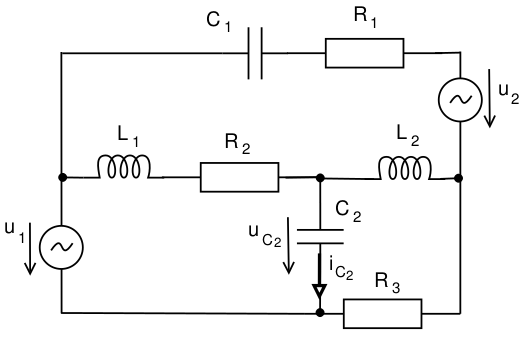
\includegraphics[width=10cm]{circuit_4.png}
		\end{center}
\end{figure}

\begin{center}

	{\textbf{\LARGE !!!TODO!!!}}
	
\end{center}

\newpage

\maketitle
\section{Príklad č.5}
	
\maketitle
\subsection{Zadanie}
Zostavte diferenciálnu rovnicu popisujúcu chovanie obvodu na obrázku, ďalej ju
upravte dosadením hodnôt parametrov. Vypočítajte analytické riešenie $u_{C}$ = $f(t)$.
Vykonajte kontrolu výpočtu dosadením do zostavenej diferenciálnej rovnice.

\begin{table}[h]
	\begin{center}		
		\begin{tabular}{|c|c|c|c|}
				\hline
				sk. & $C$ [$F$] & $R$ [$\Omega$] &  $u_{C}$(0) [$V$] \\
				\hline
				B & 10 & 20 & 8  \\
				\hline
		\end{tabular}
	\end{center}
\end{table}

\begin{figure}[h]
		\begin{center}
			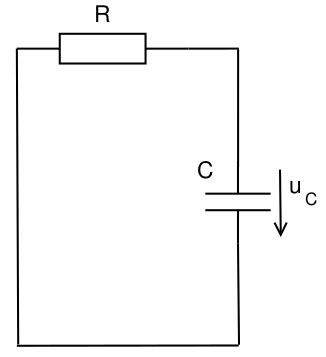
\includegraphics[width=10cm]{circuit_5.png}
		\end{center}
\end{figure}

\maketitle
\subsection{Postup diferenciálnej rovnice}

1.Poznznáme $R,C,u_{C}(0)$ a vieme vyjadriť:
\begin{eqnarray*}
	A : I &= &  \frac{U_{R}}{R} \\
	I &= & I_{C} = I_{R} \\ \\
	U_{R} + U_{C} &= & 0 \implies U_{R} = -U_{C} \\
\end{eqnarray*}

2.Ďalej určíme počiatočnú podmienku $U_{c}(0) = U_{C_{p}}$ a zostavíme ďalšiu 

rovnicu
\begin{eqnarray*}
	B : U'_{C} = \frac{1}{C} * I_{C} \\
\end{eqnarray*}

\maketitle
\subsection{Výsledok 1}

3.Dosadíme rovnicu $A$ do $B$ a určíme diferenciálnu rovnicu prvého rádu
\begin{eqnarray*}
	U'_{C} &= & \frac{1}{C} * \frac{U_{R}}{R} \\
	U'_{C} &= & \frac{U_{R}}{R*C} \\
	U'_{C} &= & -\frac{U_{C}}{R*C} = -\frac{U_{C}}{200}\\ 
\end{eqnarray*}

\maketitle
\subsection{Postup analytického riešenia}

1.Vyjadriť charakteristickú rovnicu
\begin{eqnarray*}
	Pozn.: &U'_{C} \rightarrow \lambda & \\
	&U_{C} \rightarrow 1 & \\
\end{eqnarray*}
\begin{eqnarray*}
	U'_{C} &=  & -\frac{U_{C}}{R*C}  \\
	\lambda &= & -\frac{1}{R*C}  \\
	\lambda &= & -\frac{1}{20*10}  \\
	\lambda &= & -\frac{1}{200}  \\
\end{eqnarray*}

2.Očakávaný tvar rovnice
\begin{eqnarray*}
	u_{C}(t) = k(t) * e^{\lambda \ * \ t} \\
	u_{C}(t) = k(t) * e^{-\frac{t}{200}} \\	
\end{eqnarray*}

3.Zderivujeme rovnicu
\begin{eqnarray*}
	U_{C}' = k'(t) * e^{-\frac{t}{200}} + k(t) * e^{-\frac{t}{200} * (-\frac{1}{200})} \\
\end{eqnarray*}

4.Dosadíme $U_{C}'$ a $U_{C}$ do rovnice $U_{C}' + \frac{U_{C}}{R * C} = 0$ 
\begin{eqnarray*}
	k'(t) * e^{-\frac{t}{200}} - \frac{k(t) * e^{-\frac{t}{200}}}{200} + \frac{k(t) * e^{-\frac{t}{200}}}{200} = 0 \\
\end{eqnarray*}

5.Vyjadríme $k'(t)$
\begin{eqnarray*}
	k'(t) * e^{-\frac{t}{200}} = 0 \\
\end{eqnarray*}

6.Zintegrujeme $k'(t)$
\begin{eqnarray*}
	\int k'(t) \\
	k(t) = 0 + k \\
\end{eqnarray*}

7.Dosadíme $k(t)$ do očakávaného riešenia (bod č.2)
\begin{eqnarray*}
	u_{C}(t) = k * e^{-\frac{t}{200}} \\
\end{eqnarray*}

8.Dosadíme počiatočnú podmienku $U_{C}(0) = U_{C_{p}}$
\begin{eqnarray*}
	U_{C_{p}} &= &k * e^{-\frac{t}{200}} = k * e^0 = k * 1 \\
	U_{C_{p}} &= &k \\
\end{eqnarray*}

\maketitle
\subsection{Výsledok 2}

9.Výsledná rovnica pre $u_{C}(t)$
\begin{eqnarray*}
	Vieme : u_{C}(0) &= & U_{C_{p}} * e^{-\frac{t}{200}} \\
	U_{C_{p}} &= & 8 \\
\end{eqnarray*}
\begin{eqnarray*}
	u_{C}(t) = 8 * e^{-\frac{t}{200}} \\
\end{eqnarray*}

10.Urobíme skúšku správnosti dosadením $U_{C}'$ a $U_{C}$ do pôvodnej rovnice 

$(t = 0)$
\begin{eqnarray*}
	U_{C}(0) &= &U_{C_{p}} * e^{-\frac{t}{R \ * \ C}} \\ \\
	U'_{C} &= &-\frac{U_{C}}{R*C} \\ \\
	-\frac{U_{C_{p}}}{R*C} *  e^{-\frac{t}{R \ * \ C}} &= &-\frac{U_{C_{p}}}{R*C} *  e^{-\frac{t}{R \ * \ C}} \\ \\
	-\frac{U_{C_{p}}}{R*C} &= &-\frac{U_{C_{p}}}{R*C} \\ \\
	-\frac{8}{20 * 10} &= &-\frac{8}{20 * 10} \\ \\
	-0.04 &= & -0.04 \\
\end{eqnarray*}


\newpage

\maketitle
\section{Tabuľka výsledkov}

\begin{table}[h]
	\begin{center}		
		\begin{tabular}{|c|c|c|}
				\hline
				pr.č & sk. & výsledok \\
				\hline
				1 & D & \makecell{$U_{R_{3}} = 73.5019[V]$ \\  $I_{R_{3}} = 0.2227[A]$} \\
				\hline
				2 & B & \makecell{$U_{R_{1}} = 1.4750[V]$ \\ $I_{R_{1}} = 0.0295[A]$} \\
				\hline
				3 & G & \makecell{$U_{R_{3}} = 2.4[V]$ \\ $I_{R_{3}} = 0.04528[A]$} \\
				\hline
				4 & D & \makecell{$!!!TODO!!!$} \\
				\hline
				5 & B & \makecell{$U_{C}' = -\frac{U_{C}}{200}$ \\ $u_{C}(t) = 8 * e^-\frac{t}{200}$} \\
				\hline
		\end{tabular}
	
	\end{center}
\end{table}

\end{document}
 